\section{Auswertung}
\subsection{Bestimmung der Relaxationszeit}  %--> idk wie wir layout mache wollen/section gerüst usw
Zur Bestimmung der vorher definierten Relaxationszeit $\tau = RC$ wird der Entladungsvorgung des Kondensators untersucht.
Dazu werden die gemessenen Spannungen $U_{C}$ bei entsprechender Zeit $t$ in einem halblogarithmischen Diagramm dargestellt.
Anschließend folgt die Annährung einer linearen Ausgleichsgerade durch Python, mit einem charakteristischen Steigungsparamter $a$
der Form $1/RC$. 
Die ermittelte Ausgleichsgerade hat also die Form.
\begin{equation}
    \text{ln}(U_{C}(t)) = a \cdot t + b
\end{equation}
Die Parameter der Gerade lauten.
 \begin{align*}
     a &= \SI{-80.432(5253)}{\si{\per\second}} \\
     b &= \SI{0.095(0123)}{}
 \end{align*}
Der Vergleich mit der Gleichung \eqref{eqn:gerade} zeigt nochmal die Verbindung zwischen $a$ und $\tau$. Die Relaxationszeit ist folglich.
\begin{equation}
\tau = RC = - \frac{1}{a} = \SI{12.4(8)}{\milli\second}
\end{equation}
Der Fehler ergibt sich aus einer Fehlerfortpflanzung welche bestimmt werden kann durch.
\begin{equation}
\increment \tau = \sqrt{\left( \frac{\partial \tau}{\partial a}\right)^{2} \cdot (\increment a)^{2}} = \left( \frac{\increment a}{a^{2}}\right) 
\end{equation}
\begin{figure}
    \centering 
    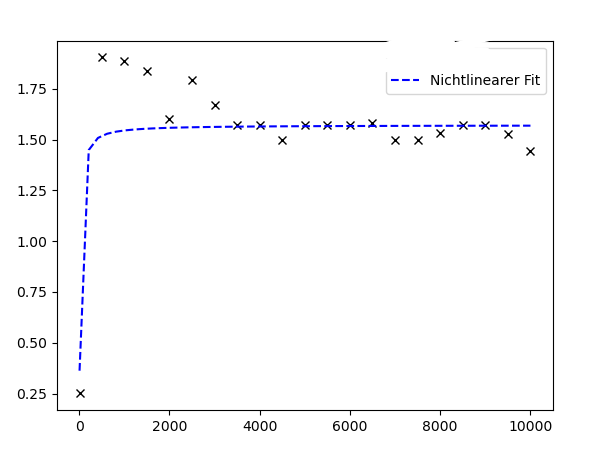
\includegraphics[width=\textwidth]{build/plot1.pdf}
    \caption{Messwerte der Entladungskurve in halblogarithmischer Darstellung mit Ausgleichsgeraden.}
    \label{plt:plot1}
\end{figure} 

\subsection{Frequenzabhängige Amplitudenmessung und Ausgleichsrechnung}

Alternativ zur Aufnahme von Auf- und Entladungskurven lässt sich das Relaxationsverhalten auch bei anliegenden Wechselspannung ermitteln.
Dabei wird die Wechselspannung auf eine Spannungsamplitude $U_{0}$ eingestellt und bei verschiedenen Frequenzen $f$ wird die Kondensatorspannungsamplitude $A(\omega)$ notiert.
Die zugehörigen Messgrößen sind in der Tabelle \ref{tab:freq} notiert und die Generatorspannungsamplitude betrug $U_{0} = \SI{11}{\volt}$.
\\
Die Gleichung \eqref{eqn:yeahyeah} liefert anschließend den Zusammenhang zwischen der Amplitude $A(\omega)$, Frequenz $f$ und Relaxationszeit $\tau$.
Durch eine nichtlineare Ausgleichsrechnung kann die Relaxationszeit nun aus den Messwerten bestimmt werden, dazu wird die Gleichung zunächst durch $U_{0}$ geteilt.
\begin{equation}
    \label{eqn:yikers}
    \frac{A(\omega)}{U_{0}} = \frac{1}{\sqrt{1+(\omega \tau)^{2}}}
\end{equation}
Ein Curvefit dieser angepassten Wertepaare liefert die Relaxationszeit.
\begin{equation*}
\tau = \SI{16.4(4)}{\milli\second}
\end{equation*}
Die Ausgleichsfunktion welche die Form von Gleichung \eqref{eqn:yikers} hat, lässt sich zusammen mit den Messwerten in einem Diagramm darstellen. In Diagramm \ref{fig:plot5}
ist eine logarithmische und in \ref{fig:plot4} eine linaere Darstellung abgebildet. 
\begin{figure}
    \centering 
    \includegraphics[width=\textwidth]{build/plot5.pdf}
    \caption{Frequenzabhängige Amplituden und Ausgleichsrechnung in logarithmischer Darstellung.}
    \label{fig:plot5}
\end{figure} 
\begin{figure}
    \centering 
    \includegraphics[width=\textwidth]{build/plot4.pdf}
    \caption{Frequenzabhängige Amplituden und Ausgleichsrechnung in linearer Darstellung.}
    \label{fig:plot4}
\end{figure} 
Zu erkennen ist also eine systematische Abweichung, des errechneten Wertes der Entladungskurve, von.
\begin{equation}
\tau_{\si{\percent}} = \SI{24.4(18)}{\percent}
\end{equation}
%Bei größer werdenden Frequenzen nimmt also die Spannungsamplitude am Kondensators ab, dies bestätigt die Eigenschaft des 
%RC-Kreises als Tiefpassfilter. Er lässt kleine Frequenzen ungehindert hindurch aber hohe Frequenzen werden unterdrückt.
\subsection{Phasenverschiebung der Kondensatorspannung}
Aus der dritten Messreihe können die Phasenverschiebung durch die Gleichung \eqref{eqn:phi} errechnet werden. Diese sind zusammen
mit den Frequenzen $f$ in der Tabelle \ref{tab:freq} angegeben.
Der Zusammenhang aus \eqref{eqn:sadge} liefert uns eine enstprechend dritte Art zur Bestimmung der Zeitkonstante $RC$.
\begin{equation}
    \phi(\omega) = \text{arctan}(-\omega RC)
\end{equation}
Analog zu den vorherigen Teil wird hier eine nichtlineare Ausgleichsfunktion mit Hilfe eines Curvefit in Python gefunden.
Der Parameter $\tau$ enstpricht der Zeitkonstante $RC$ und beträgt.
\begin{equation}
    \tau = \SI{37.9(07)}{\ms}
\end{equation}
Die abbildene Funktion ist in Abbildung \ref{fig:plttausend} dargestellt. Im Vergleich zu den anderen Messreihen fällt hier eine besonders
große Differenz zur optimalen Zeitkonstante auf.
\begin{equation*}
    \label{eqn:Mp1kompletterMuell}
    \tau_{\si{\percent}} = \SI{131.1(71)}{\percent}
\end{equation*}
\begin{figure}
    \centering 
    \includegraphics[width=\textwidth]{build/plot6.pdf}
    \caption{Frequenzabhängige Phasenverschiebung und Ausgleichsrechnung in nicht linearer Darstellung.}
    \label{fig:plttausend}
\end{figure} 

\subsection{Abhängigkeit der Relativamplitude von der Phase}